\documentclass{article}
\setlength{\parskip}{5pt} % esp. entre parrafos
\setlength{\parindent}{0pt} % esp. al inicio de un parrafo
\usepackage{amsmath} % mates
\usepackage[sort&compress,numbers]{natbib} % referencias
\usepackage{url} % que las URLs se vean lindos
\usepackage[top=25mm,left=20mm,right=20mm,bottom=25mm]{geometry} % margenes
\usepackage{hyperref} % ligas de URLs
\usepackage{graphicx} % poner figuras
\usepackage[spanish]{babel} % otros idiomas
\usepackage[utf8]{inputenc} % alparecer son los acentos
\documentclass[12pt,letterpaper]{article}
\usepackage[utf8]{inputenc}
\usepackage{tikz}
\usetikzlibrary{trees}
\usepackage[spanish, es-nodecimaldot]{babel}
\usepackage{color}
\usepackage{algorithm}
\usepackage[noend]{algpseudocode}
\renewcommand{\algorithmicrequire}{\textbf{Entrada:}}
\renewcommand{\algorithmicensure}{\textbf{Salida:}}
\usepackage{subcaption}
\usepackage{amsfonts}
\usepackage{hyperref}
 \hypersetup{
     colorlinks=true,
     linkcolor=blue,
     filecolor=teal,
     citecolor = gray,      
     urlcolor=blue,
     }
\usepackage{amssymb}
\usepackage{listings}
\usepackage{color}
\author{I E G} % author
\title{Práctica 9 : interacciones entre partículas} % titulo
\date{\today}

\begin{document} % inicia contenido

\maketitle % cabecera

\begin{abstract} % resumen
Se trabaja con un modelo simplificado de simulación para fenómenos de atracción y repulsión figura \ref{fig1} como en la \href{https://github.com/IsaacEstrada159/simulacion/blob/master/P09/elisagif/p9p.gif}{animación} 1, agregando para la práctica a cada partícula una masa \cite{elis9} que cause fuerzas gravitacionales entre si además de cargas eléctricas y analizar su distribución de las velocidades, magnitud de la carga, masa y sus posiciones.

\begin{figure} [h!]
 	\centering
 	\begin{subfigure}[b]{0.40\linewidth}
 		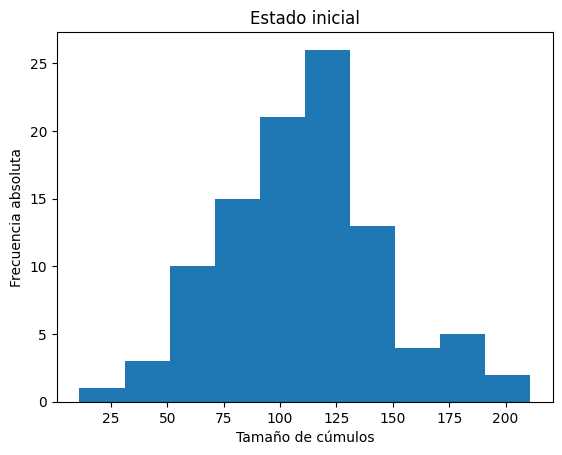
\includegraphics[width=\linewidth]{fig1.png}
 		 \caption{Paso 1.}
 		\label{3d}
 	\end{subfigure}
 	\begin{subfigure}[b]{0.40\linewidth}
 		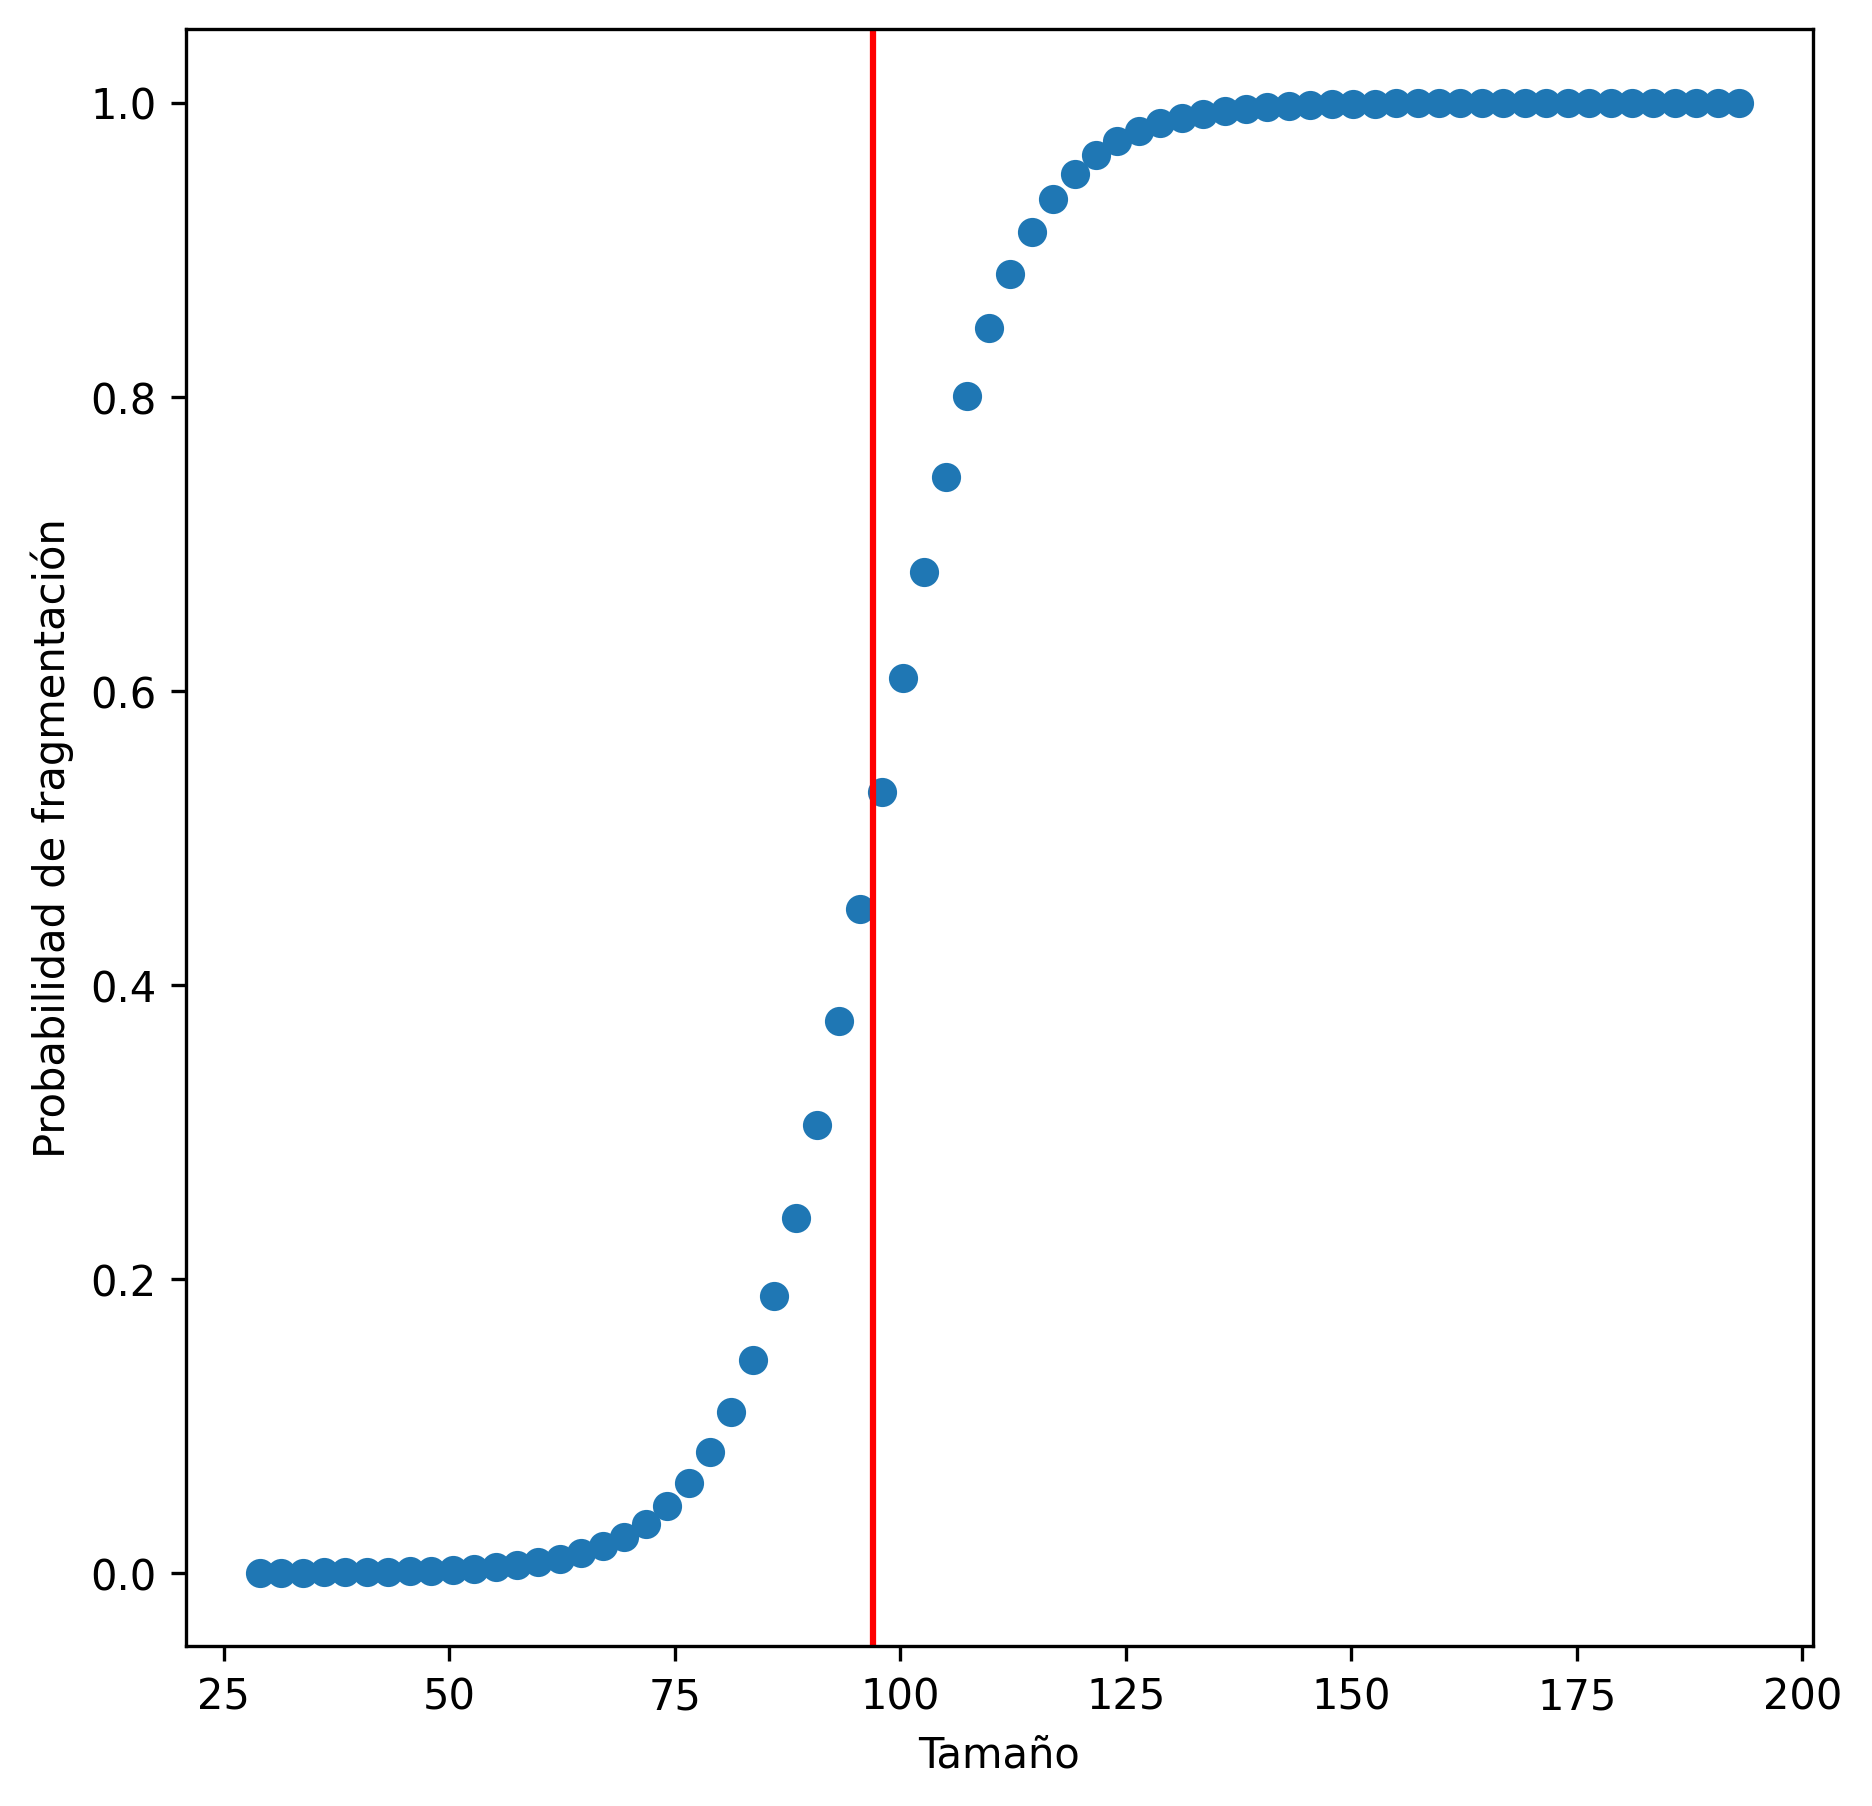
\includegraphics[width=\linewidth]{fig2.png}
 		 \caption{Paso 18.}
 		\label{levelplot}
 	\end{subfigure}
 	 	\begin{subfigure}[b]{0.40\linewidth}
 		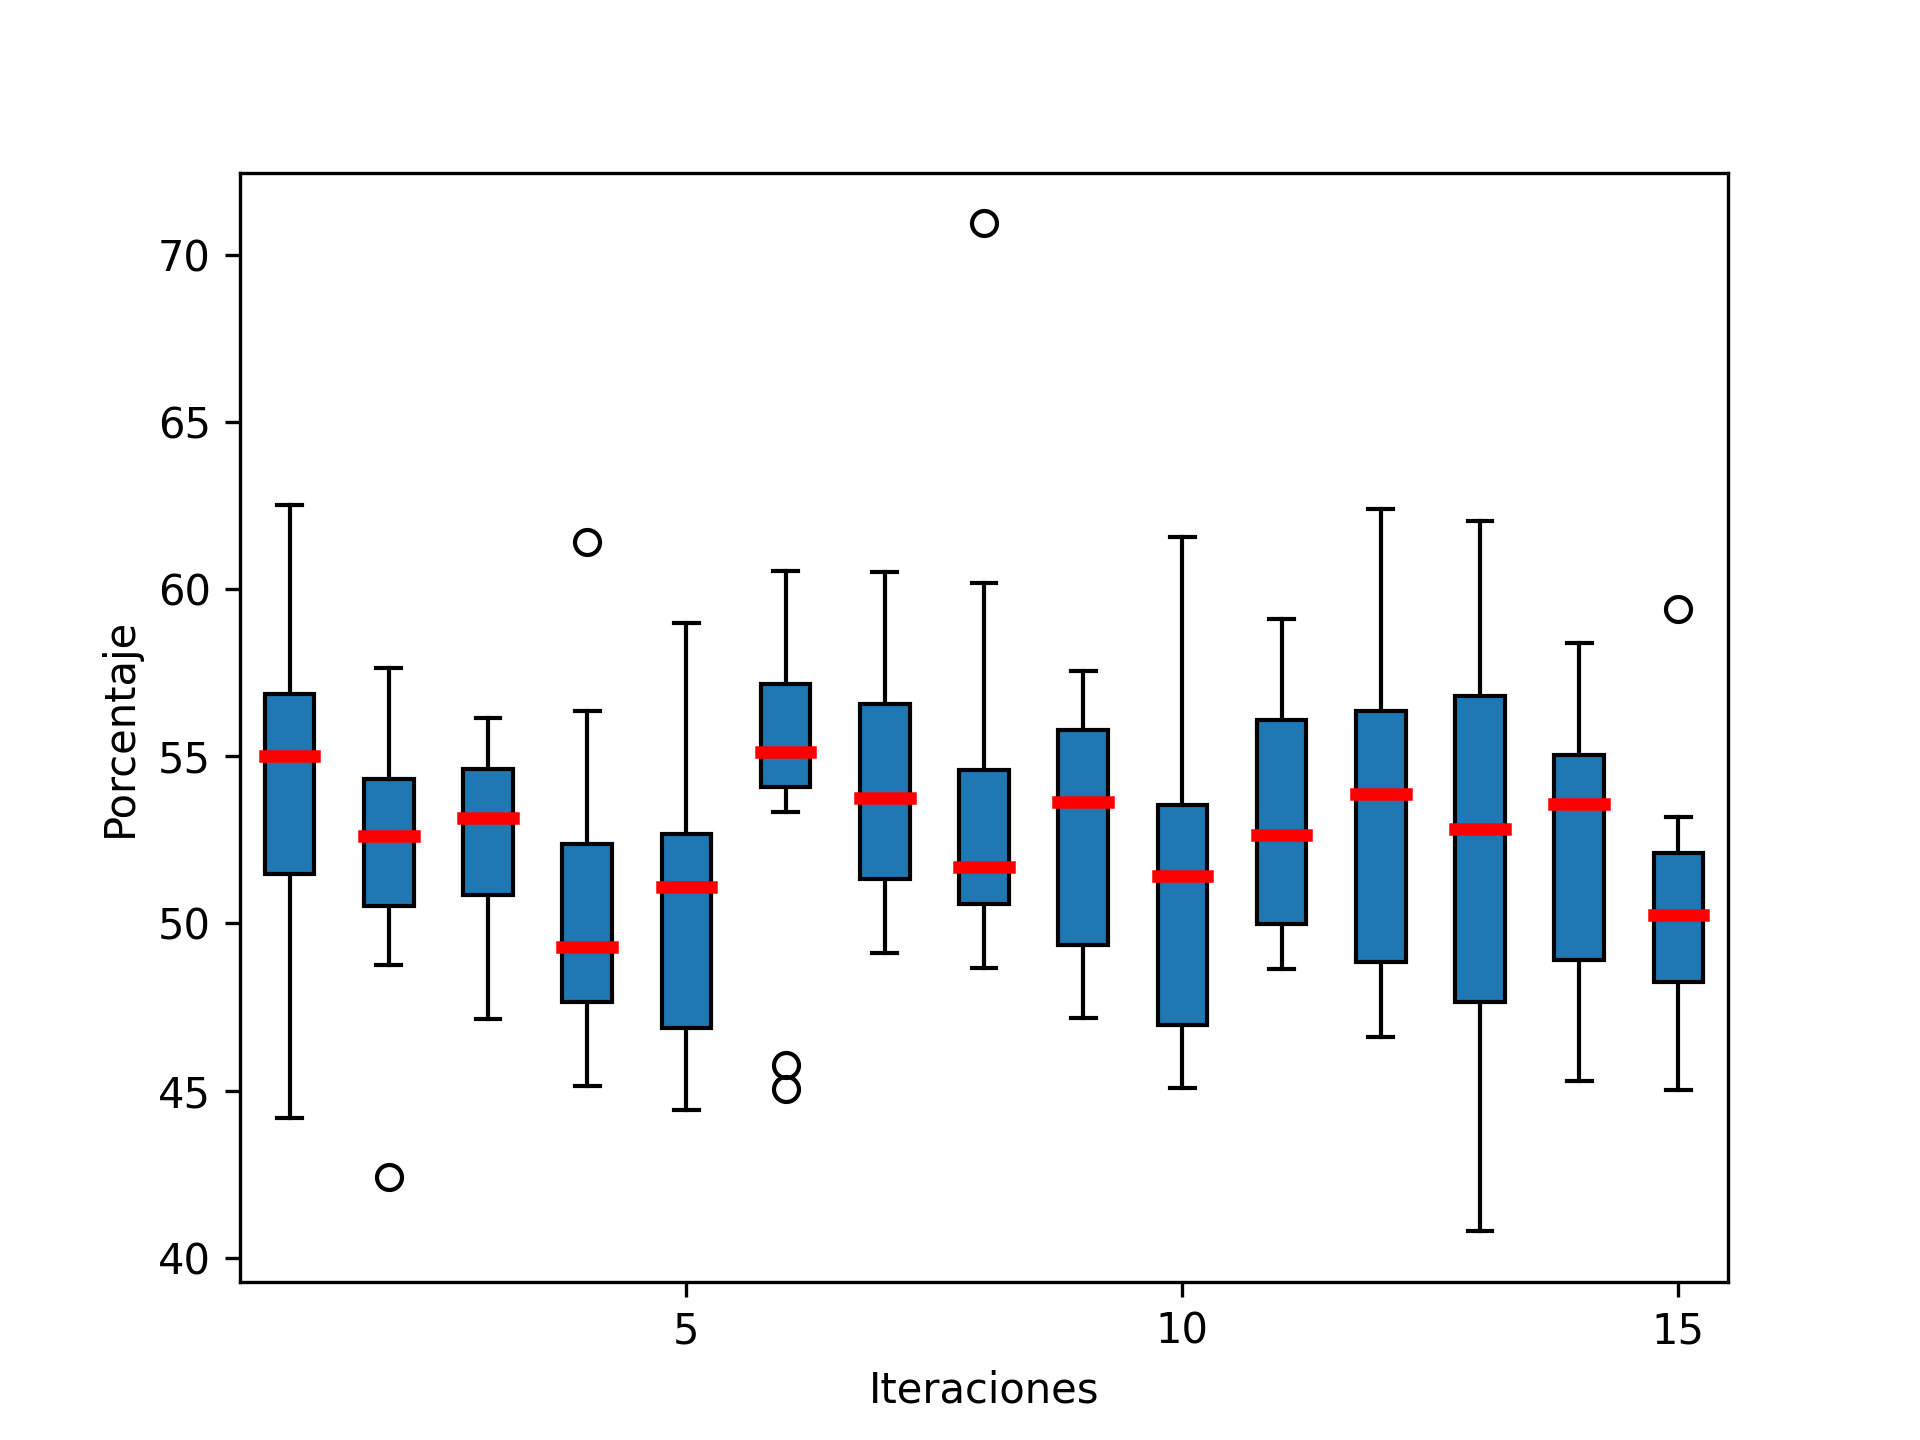
\includegraphics[width=\linewidth]{fig3.png}
 		 \caption{Paso 50.}
 		\label{levelplot}
 	\end{subfigure}
 	\caption{Gráficas atracción y repulsión.}  	
\label{fig1}
 \end{figure}




\end{abstract}


\section{Desarrollo}
Para la simulación se usa el paquete estadístico R versión 4.0.2 \cite{R} para correr el código previamente reportado \cite{elis9} donde las interacciones entre las partículas son posicionadas normalmente al azar en un cuadro unitario \cite{Fab3, cae2} además de que estas poseen una carga que causa sus debidas fuerzas entre ellas, también se añade una variable masa a las partículas que afecte la interacción de las mismas. Se utilizan 20 partículas que se afectan entre sí para que la simulación  pueda ser observada dentro de cuadro unitario con la justificación de observar el fenómeno de manera justamente visible en las gráficas generadas.


\section{Experimento}
En la figura \ref{fig2} se muestra la simulación donde interactúan 20 partículas, las masas se ven representadas con círculos de diferente tamaño y el color identifican su carga. Para observar de mejor manera la simulación del experimento se aprecia en la \href{https://github.com/IsaacEstrada159/simulacion/blob/master/P09/buenos/ezgif.com-gif-maker%20(1).gif}{animación} 2.

\begin{figure} [h!]
 	\centering
 	\begin{subfigure}[b]{0.40\linewidth}
 		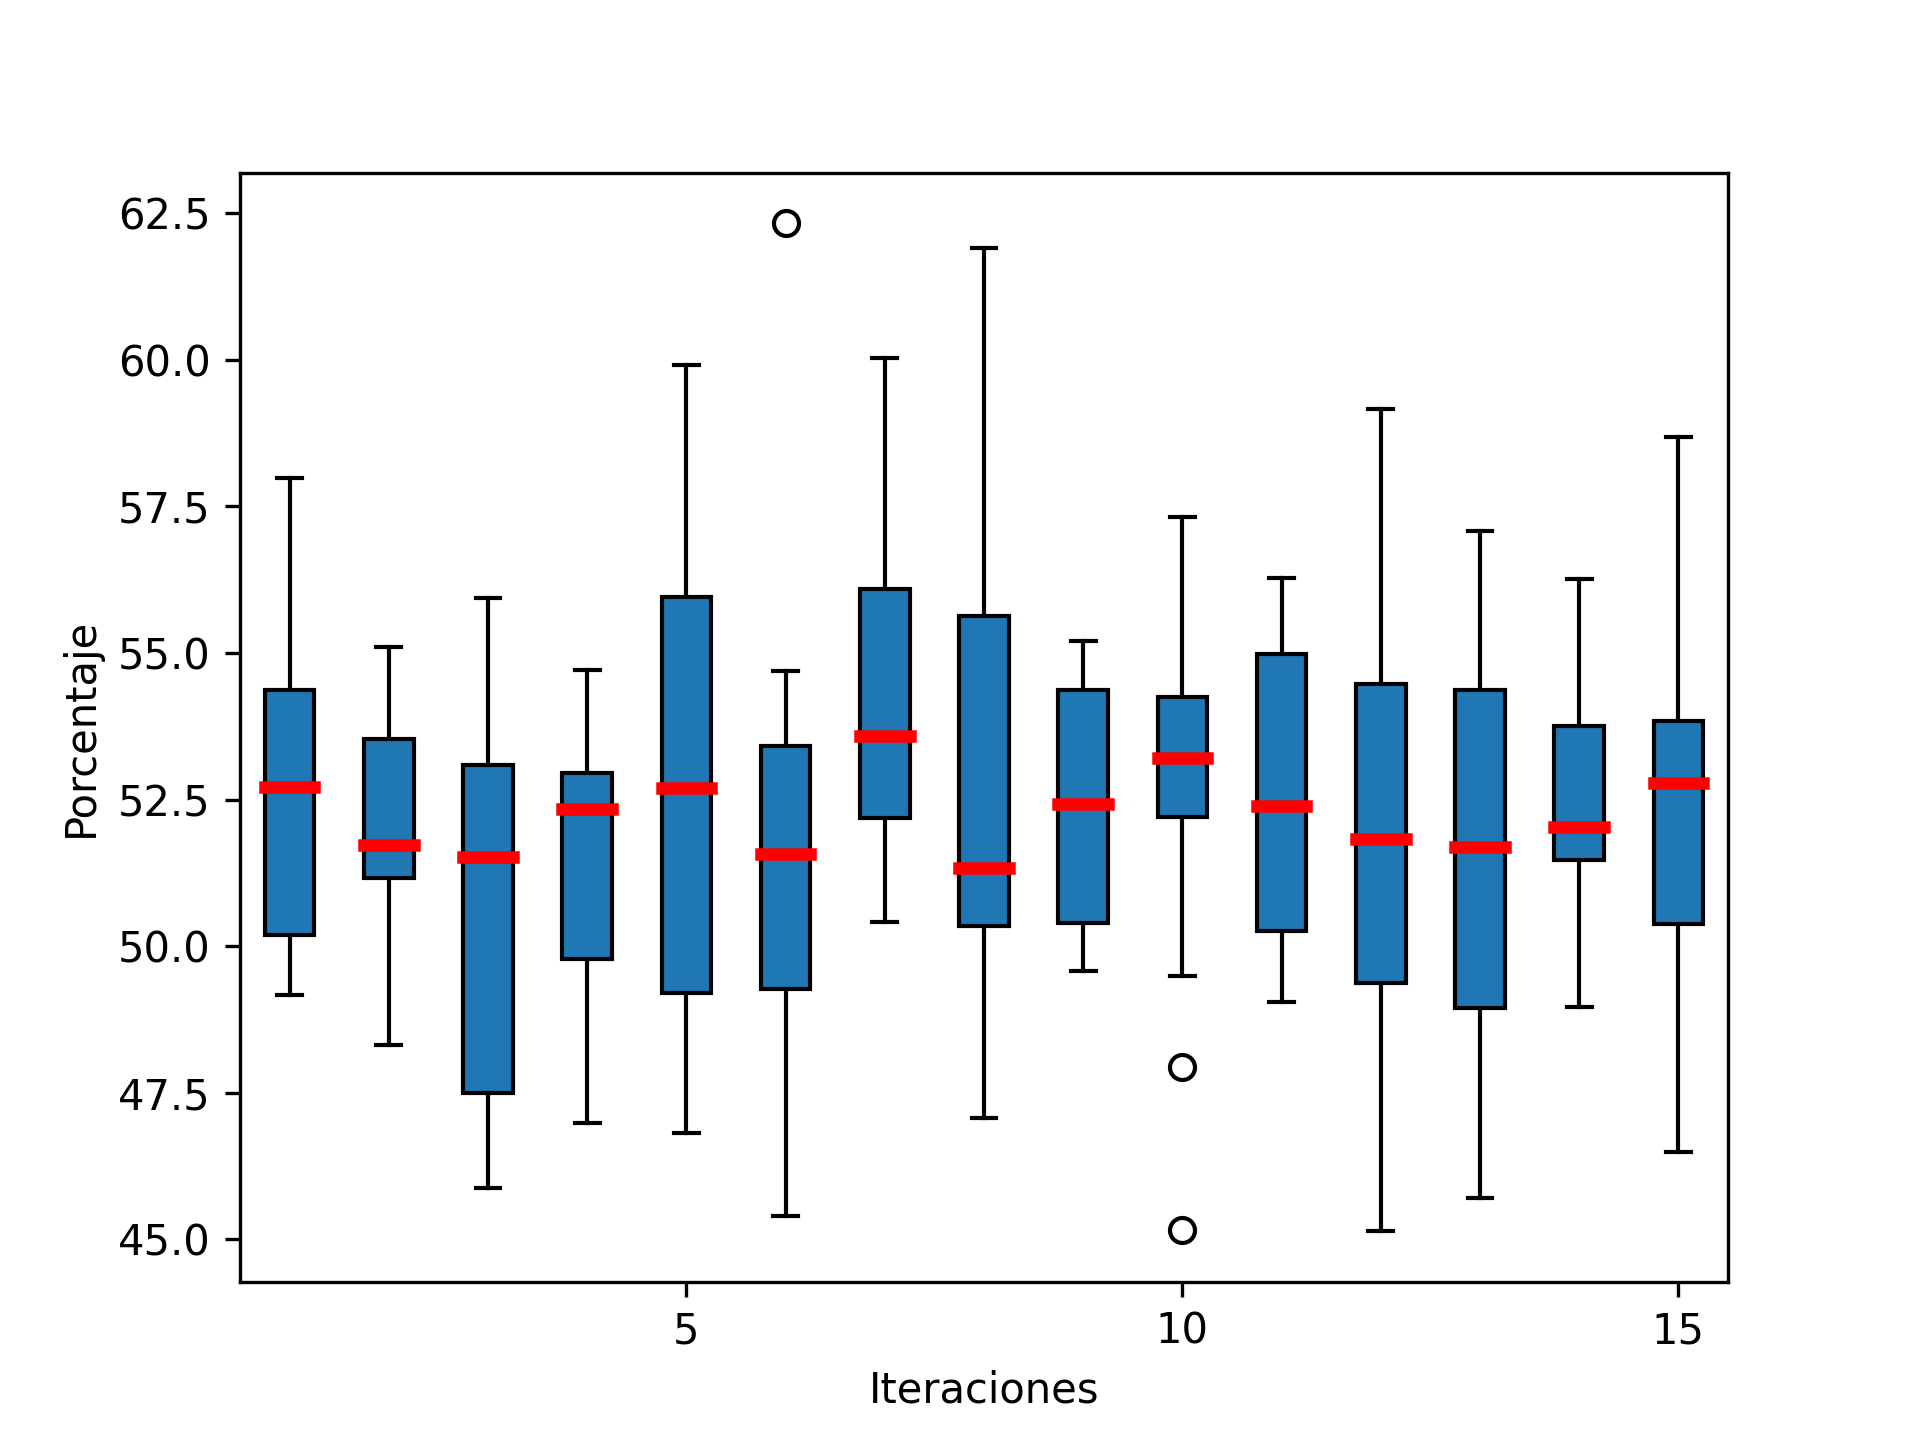
\includegraphics[width=\linewidth]{fig4.png}
 		 \caption{Paso 1.}
 		\label{3d}
 	\end{subfigure}
 	\begin{subfigure}[b]{0.40\linewidth}
 		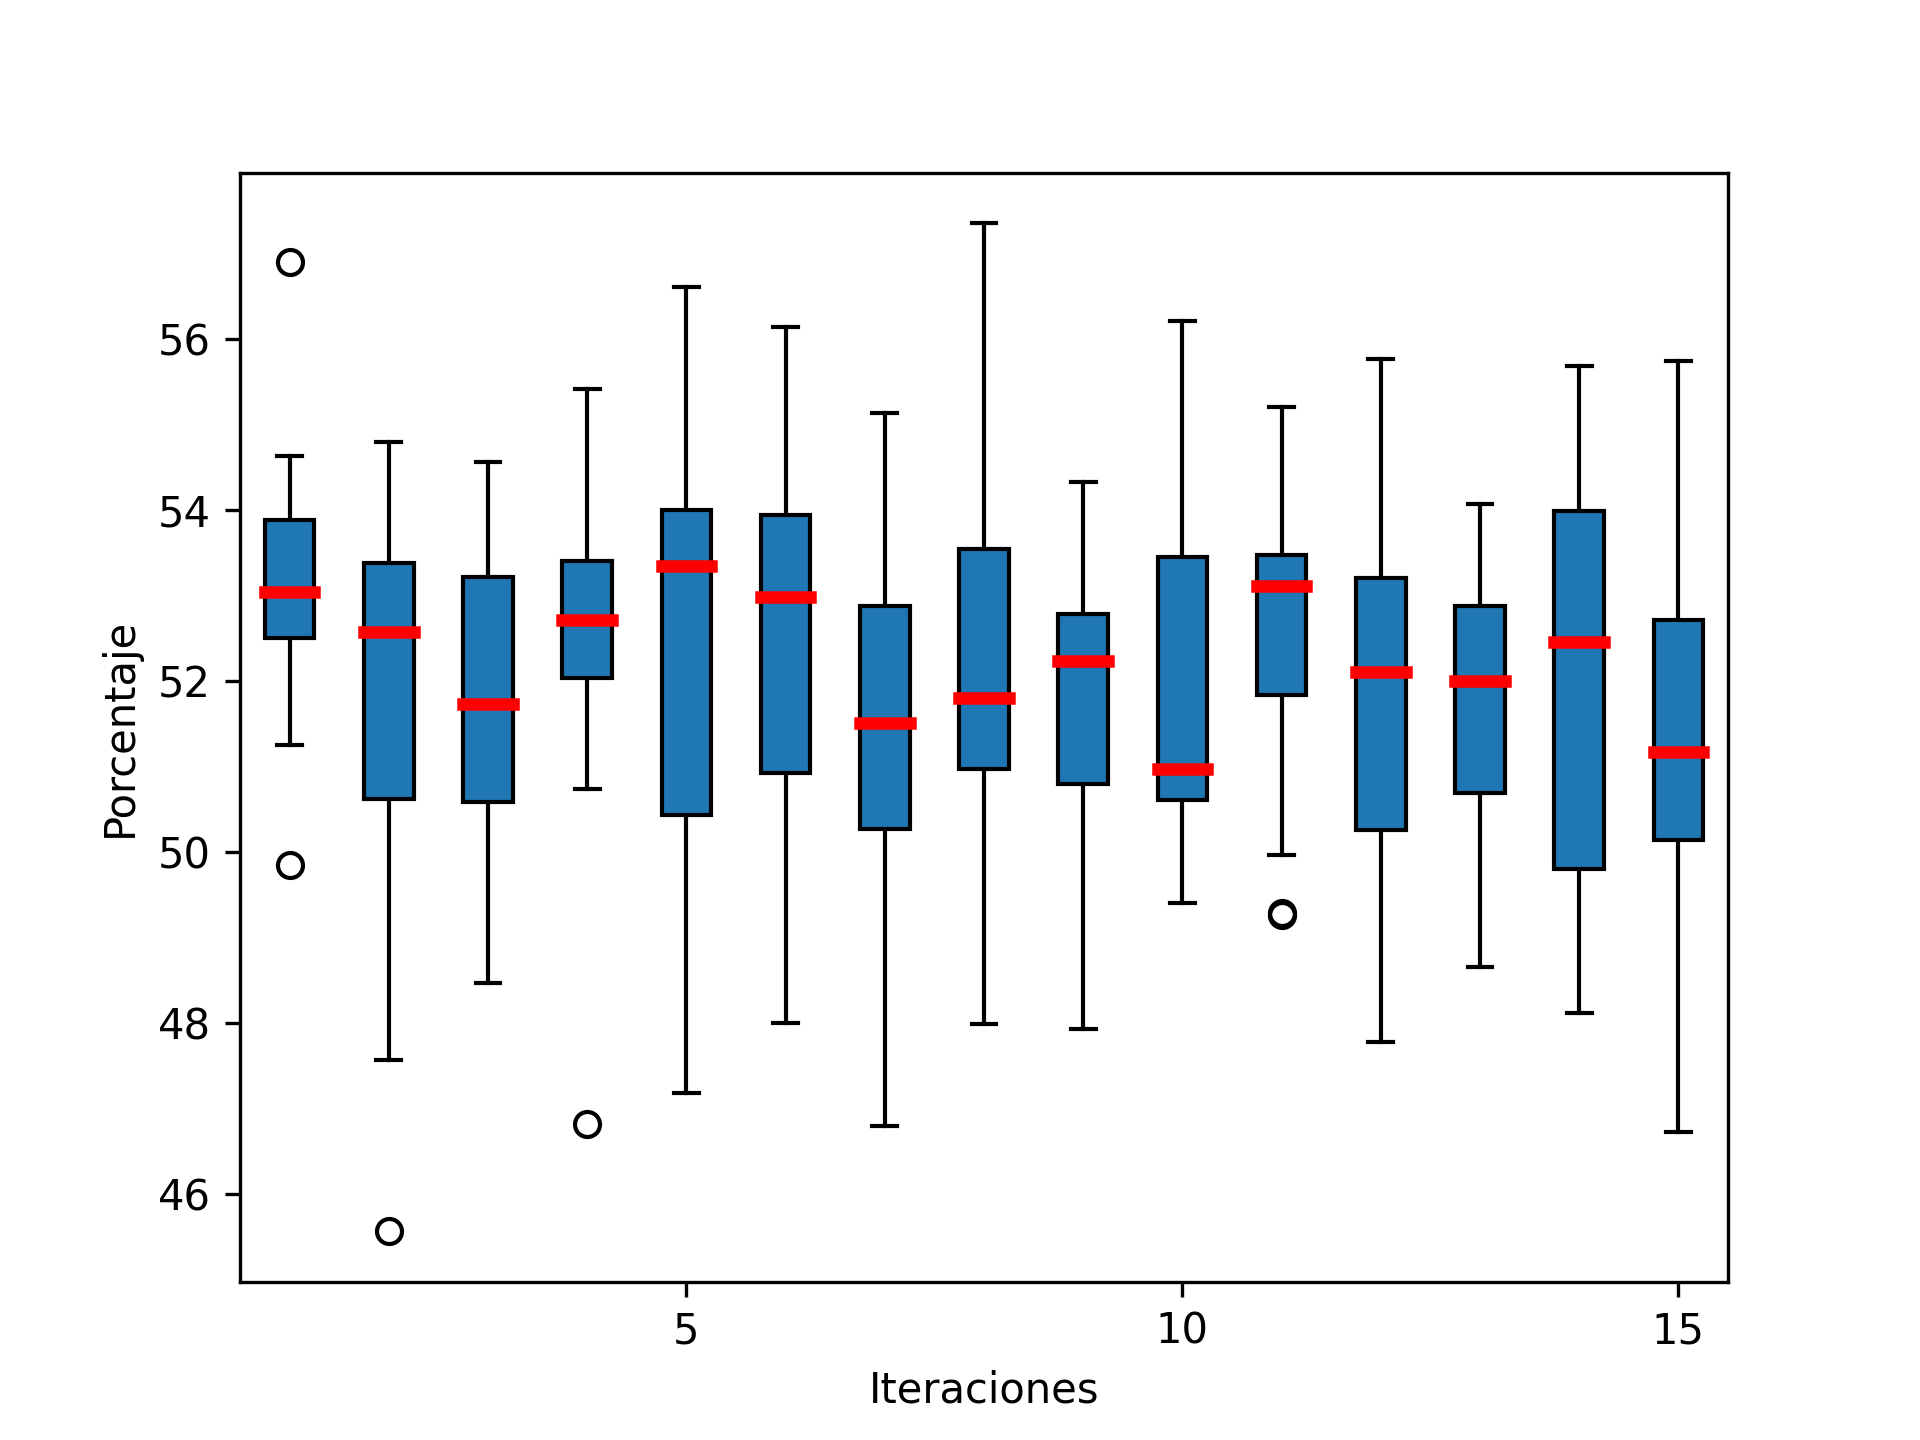
\includegraphics[width=\linewidth]{fig5.png}
 		 \caption{Paso 25.}
 		\label{levelplot}
 	\end{subfigure}
 	 	\begin{subfigure}[b]{0.40\linewidth}
 		\includegraphics[width=\linewidth]{fig6.png}
 		 \caption{Paso 100.}
 		\label{levelplot}
 	\end{subfigure}
 	\caption{Simulación con carga y masa.}  	
\label{fig2}
 \end{figure}

En la figura \ref{fig3} se muestran los histogramas de los pasos 1 y 100 de las posiciones en $x$ y $y$ donde se observa con esta información obtenida en histogramas y gráficos de dispersión de los factores: posición inicial y final, carga, masa y velocidad, al final dichos gráficos se observan como la carga y la masa afectan la velocidad. 

\begin{figure} [h!]
 	\centering
 	\begin{subfigure}[b]{0.40\linewidth}
 		\includegraphics[width=75mm]{fig7.png}
 		 \caption{Paso 1.}
 		\label{3d}
 	\end{subfigure}
 	\begin{subfigure}[b]{0.40\linewidth}
 		\includegraphics[width=75mm]{fig8.png}
 		 \caption{Paso 100.}
 		\label{levelplot}
 	\end{subfigure}
 	\caption{Matrices de dispersión de las partículas en los pasos 1 y 100.}  	
\label{fig3}
 \end{figure}
 
\section{Conclusiones} 

En conclusión, la masa de las partículas afecta sobre la velocidad que es más  influyente a lo largo de las iteraciones mayores estando inversamente relacionadas.



\bibliography{bib}
\bibliographystyle{plainnat}

\end{document}